\documentclass[12pt]{article}

%IMPORTS
\usepackage[catalan]{babel}
\usepackage[utf8]{inputenc}
\usepackage{graphicx}
\usepackage{wrapfig}
\usepackage{amsmath}
\usepackage{amssymb}
\usepackage{ragged2e} 
\usepackage{subfig}
\usepackage{caption}
\usepackage{subcaption}
\usepackage[usenames]{color}
\usepackage{xcolor}
\usepackage{float}
\usepackage{chngcntr}
\usepackage{ragged2e}
\usepackage{multirow}
\usepackage{multicol}
\usepackage{vmargin}
\usepackage{hyperref}
\usepackage{subfigure}
\usepackage{url}

\definecolor{blue(ncs)}{rgb}{0.0, 0.53, 0.74}
\setlength{\columnsep}{70pt}

\begin{document}

\begin{titlepage}
    \centering
    \vspace{4cm}
    {\bfseries\LARGE Universitat Autònoma de Barcelona\newline Facultat de Ciències\par}
    \vspace{6cm}
    {\scshape\Huge Modelització i Inferencia Pràctica 1 \par} 
    \vspace{2cm}
    {\Large \itshape Autor: \par}
    {\Large Gerard Lahuerta Martín\par}
    {\small NIU: 1601350\par}
    \vspace{3cm}
    {\Large 18 de Novembre del 2021\par}
\end{titlepage}

\justifying


\newpage
\setcounter{page}{2}
\pagestyle{plain}
\tableofcontents
\cleardoublepage
\addcontentsline{}{chapter}{}
\section{Presentació del problema}
Suposa una mostra aleatòria $X_1, \cdots , X_n$ $\sim$ $Binomial (1, p)$. Considera l'estimador
\begin{equation*}
T = \frac{\sqrt{n}}{2(n+\sqrt{n})}+\frac{1}{n+\sqrt{n}}\sum^{n}_{i=1}{X_i}
\end{equation*}

per al paràmetre desconegut $p \in (0, 1)$.\\
\begin{enumerate}
\item [(a)] És $T$ un estimador no esbiaixat per a $p \in (0, 1)$? Justifica la teva resposta.
\item [(b)] Calcula el $MSE$ de $T$ i fes una representació de $T$ com a funció del paràmetre desconegut
$p \in (0, 1)$ considerant $n = 10$ i $n = 50$. Què observes?
\item [(c)] És $T$ consistent? I asimptòticament no esbiaixat? Justifica les teves respostes.
\end{enumerate}

\newpage
\section{Resolució del primer apartat} \label{cap:res1}
$T$ serà un estimador de $X_i$ si empíricament obtenim el valor teòric de l'esperança de $X_i, \forall i\in\{1,\cdots,n\}$; és a dir, $T$ serà un estimador no esbiaixat si i només si
$$Bias(T) = 0 \Leftrightarrow E(X_i) - E(T) = 0 \Leftrightarrow E(X_i) = E(T) \hspace{0.5em} \forall i\in\{1,\cdots,n\}$$
Escollim per a exemple $i=1$ (ja que dona igual quina variable aleatòria escollim perquè són independents i idènticament distribuïdes). Sabem que \\$E\left(X\sim Binomial (1, p)\hspace{0.5}\right) = E(Y\sim Bernoulli(p)\hspace{0.5})=p$.\\\\
\textbf{Calculem el valor de \textit{E(T)}:}\\
\begin{equation*}

E(T) =E\left(\frac{\sqrt{n}}{2(n+\sqrt{n})}+\frac{1}{n+\sqrt{n}}\sum^{n}_{i=1}{X_i}\right)=E\left(\frac{\sqrt{n}}{2(n+\sqrt{n})}\right)+E\left(\frac{1}{n+\sqrt{n}}\sum^{n}_{i=1}{X_i}\right)=
\end{equation*}
\begin{equation*}
=\frac{\sqrt{n}}{2(n+\sqrt{n})}+\frac{1}{n+\sqrt{n}}E\left(\sum^{n}_{i=1}{X_i}\right) \underset{\underset{\textbf{(\textit{I})}}{\uparrow}}{=}\frac{\sqrt{n}}{2(n+\sqrt{n})}+\frac{n}{n+\sqrt{n}}E(X_1)=
\end{equation*}
\begin{equation*}
=\frac{\sqrt{n}}{2(n+\sqrt{n})}+\frac{n}{n+\sqrt{n}}p=\frac{\sqrt{n}+2np}{2(n+\sqrt{n})}\Longrightarrow E(T)=\frac{\sqrt{n}+2np}{2(n+\sqrt{n})}
\end{equation*}
\\
(I): \textit{$X_1, \cdots , X_n$ independents i idènticament distribuïdes}\\\\
\textbf{Calculem ara el \textit{Bias(T)}}
\begin{equation*}
-Bias(T)=E(X_1)-E(T)=p-\frac{\sqrt{n}+2np}{2(n+\sqrt{n})}=\frac{2\sqrt{n}p+2np-\sqrt{n}-2np}{2(\sqrt{n}+n)} =
\end{equation*}
\begin{equation*}
=\frac{(2p-1)\sqrt{n}}{2(\sqrt{n}+n)}=\frac{2p-1}{2(1+\sqrt{n})}
\end{equation*}
Veiem de l'expressió trobada que s'anul·larà el numerador (i per tant el $Bias(T)=0$) quan $p=\frac{1}{2}$.\\
Observem, per tant, que:\\ $$\text{ \textcolor{blue}{ \boxed{ T \text{ és un estimador esbiaixat } \forall p\in [0,\frac{1}{2})\cup (\frac{1}{2},1], \text{ perquè per aquests valors } Bias(T)\neq0}}}$$
\newpage
\section{Resolució del segon Apartat}

\subsection{Càlcul del $MSE$}
Per a calcular el $MSE$ del estimador $T$ cal saber abans la seva variància, ja que $MSE(T)=V(T)-Bias^2(T)$ i el valor del $Bias(T)$ ja el tenim conegut per l'apartat anterior.\\
\textbf{Calculem el valor de \textit{V(T)}:}\\
\begin{equation*}
V(T)=V\left(\frac{\sqrt{n}}{2(n+\sqrt{n})}+\frac{1}{n+\sqrt{n}}\sum^{n}_{i=1}{X_i}\right)=\left(\frac{1}{n+\sqrt{n}}\right)^2V\left(\sum^{n}_{i=1}{X_i}\right)\underset{\underset{\textbf{(\textit{II})}}{\uparrow}}{=}
\end{equation*}
\begin{equation*}
=\frac{1}{(n+\sqrt{n})^2}nV(X_1)\underset{\underset{\textbf{(\textit{II})}}{\uparrow}}{=}\frac{np(1-p)}{(n+\sqrt{n})^2}=\frac{np(1-p)}{n^2+2n\sqrt{n}+n}=\frac{p(1-p)}{n+2\sqrt{n}+1}
\end{equation*}
\\
(II): \textit{Sabem que la variància d'una $Binomial(1,p)$ és la suma de les variàncies que té de $Bernoulli(p)$; és a dir, en aquest cas $V(X_1)=p(1-p)$}\\\\
Ja amb tota la informació necessària, calculem el valor del $MSE(T)$\\\\
\textbf{Càlcul del valor de \textit{MSE(T)}:}\\
\begin{equation*}
MSE(T)=V(T)+Bias^2(T)=\frac{p(1-p)}{n+2\sqrt{n}+1}+\left(\frac{2p-1}{2(1+\sqrt{n})}\right)^2=
\end{equation*}
\begin{equation*}
= \frac{p(1-p)}{n+2\sqrt{n}+1}+\frac{4p^2-4p+1}{4(1+2\sqrt{n}+n)} = \frac{4p(1-p)+4p^2-4p+1}{4(1+2\sqrt{n}+n)} =
\end{equation*}
\begin{equation*}
= \frac{4p -4p^2 +4p^2 -4p +1}{4(1+2\sqrt{n}+n)} = \frac{1}{4(1+2\sqrt{n}+n)} \Longrightarrow \textcolor{blue}{ \boxed{MSE(T)=\frac{1}{4(1+2\sqrt{n}+n)}}}
\end{equation*}
\newpage
\subsection{Representació de $T$}
Per tal d'observar amb més detall com és de bo l'estimador $T$, hem decidit fer un seguit de representacions mitjançant $RStudio$ i representar els resultats obtinguts. Així, podem fer-nos una idea de com interactua $T$ i si els nostres resultats teòrics obtinguts són correctes.
\subsubsection{Simulació de l'estimador $T$}
El programa que simula el comportament del nostre estimador $T$ està dividit en 4 parts:
\begin{itemize}
\item \textbf{Inicialització de les variables}\\
Declara i assigna valors a constants que utilitzarem al llarg del programa.
\begin{itemize}
\item[\rightarrow] $n=\{10,50\}$ nombre de mostres aleatòries.
\item[\rightarrow] $M=500$ nombre de simulacions a fer per cada probabilitat.
\item[\rightarrow] $p=[0,0.1,0.2,0.3,\cdots,0.9,1]$ llista de probabilitats per a fer les simulacions.
\item[\rightarrow] $sq=\sqrt{n}$ variable que farem servir per a calcular els valors de l'estimador.
\item[\rightarrow] $den=sq+n$ variable que farem servir per a calcular els valors de l'estimador.
\item[\rightarrow] $coef\_T1=\frac{sq}{2\cdot den}$ variable que farem servir per a calcular els valors de l'estimador.
\item[\rightarrow] $coef\_T2=\frac{1}{den}$ variable que farem servir per a calcular els valors de l'estimador.
\end{itemize}
\item \textbf{Declaració de les funcions}\\
Declarem la funció $T$ que farem servir durant la simulació,
inserim aquí el codi de la funció.
\begin{center}
\begin{verbatim}
T = function( x ){
return (coef_T_1 + coef_T_2*x)
}
\end{verbatim}
Funció de l'estimador $T$
\end{center}
\newpage
\item \textbf{Main del programa simulador}\\
Part principal del programa on és dur a terme les simulacions de l'estimador $T$. Inserim aquí el Main del programa
\begin{verbatim}
That = matrix(NA, length(p), M)
for (i in 1:length(p)) {
for (j in 1:M) {
That [i,j] = T(rbinom(1,n,p[i]))
}
}

MSE = (apply(That, MARGIN = 1, FUN = mean) -p)^2
MSE = MSE + apply(That, MARGIN = 1, FUN = var)

#OUTPUT
plot(p, MSE, type = "b")
\end{verbatim}
\textbf{\textit{Observació:}}\\\textit{L'output del programa és un gràfic amb el comportament de l'estimador}
\newpage\item \textbf{Output del programa: anàlisis dels gràfics}\\
Inserim aquí una petita recopilació dels outputs obtinguts.

\begin{figure}[h]
\centering
\subfloat[Simulació 1]{
\label{f:t1}
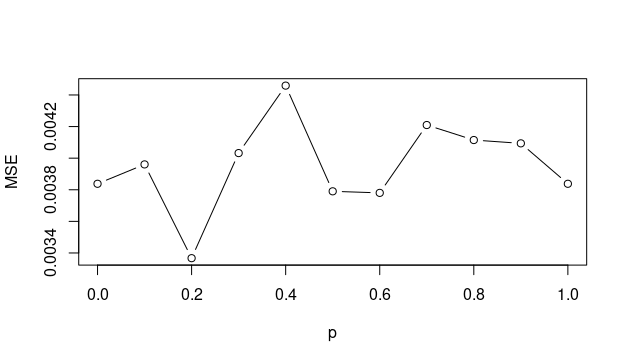
\includegraphics[width=0.5\textwidth]{t1.png}}
\subfloat[Simulació 2]{
\label{f:t2}
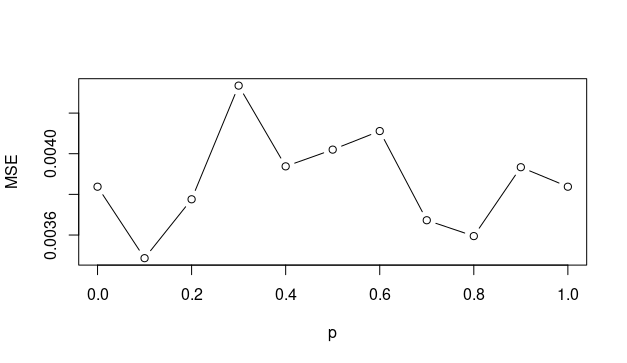
\includegraphics[width=0.5\textwidth]{t2.png}}
\caption{Gràfic per les simulacions amb $n=10$}
\label{f:t}
\end{figure}
\begin{figure}[h]
\centering
\subfloat[Simulació 1]{
\label{f:T1}
\includegraphics[width=0.5\textwidth]{T1.png}}
\subfloat[Simulació 2]{
\label{f:T2}
\includegraphics[width=0.5\textwidth]{T2.png}}
\caption{Gràfic per les simulacions amb $n=50$}
\label{f:T}
\end{figure}
\subsubsection{Conclusions extretes dels resultats obtinguts}
Dels gràfics del comportament de l'estimador $T$, deduïm que aquest no segueix cap relació amb el paràmetre $p$, ja que no dur a terme cap comportament que no sembli atzarós a mesura que augmentem el valor del paràmetre.\\ Aquest comportament confirma els càlculs obtinguts teòrics obtinguts anteriorment que deien que l'$MSE$ de l'estimador $T$ no depenia en cap moment del valor de $p$.\\ Per altra banda observem que a mesura que augmentem el valor de l'$n$, els rangs de valors que obté l'$MSE$ disminueix, apropant-se més al zero.\\ Aquest comportament també ha estat previst pels càlculs teòrics que mostraven relació entre el valor de l'$n$ i l'$MSE$ (ja que aquest paràmetre està en el denominador de la funció $MSE$ obtinguda). \\Deduïm per tant, que l'únic paràmetre rellevant per a disminuir l'$MSE$ és el nombre de Bernouillis que conformen la Binomial $X$; és a dir, el valor de $n$.
\end{itemize}

\newpage
\section{Resolució del tercer Apartat}
A partir del càlcul del $MSE(T)$ de l'apartat anterior. Calculem la consistència de l'estimador $T$ i si és o no asimptòticament esbiaixat.

\subsection{Consistencia de $T$}
Sabem que l'estimador $T$ és consistent $\Longleftrightarrow \underset{n\rightarrow\infty}{lim}MSE(T) = 0$. \\Calculem ara el límit:
\begin{equation*}
\underset{n\rightarrow\infty}{lim}MSE(T)=\underset{n\rightarrow\infty}{lim}\frac{1}{4(1+2\sqrt{n}+n)}=\frac{1}{4(\infty+2\cdot\infty)}=\frac{1}{\infty}=0\Longrightarrow
\end{equation*}
$\Longrightarrow$ \textcolor{blue}{\boxed{\text{l'estimador $T$ és consistent}}}\\
\textit{La consistència de l'estimador $T$ també s'observa a partir de les gràfiques mostrades en la pàgina anterior, on a mesura que augmenta el valor de $n$ el valor de l'$MSE$ decreix cap a $0$}

\subsection{Esbiaixat asimptòtic de $T$}
Eventualment, calculem si $\underset{n\rightarrow\infty}{lim}Bias(T)=0$, ja que $T$ serà asimptòticament no esbiaixat si compleix la condició anterior.\\
Calculem ara el límit:
\begin{equation*}
\underset{n\rightarrow\infty}{lim}Bias(T)=\underset{n\rightarrow\infty}{lim}\frac{2p-1}{2(1+\sqrt{n})}=\frac{2p-1}{2(1+\sqrt{\infty})}=\frac{2p-1}{\infty}=0 \Longrightarrow
\end{equation*}
$\Longrightarrow$
\textcolor{blue}{\boxed{\text{l'estimador $T$ és asimptòticament no esbiaixat}}}
\newpage
\section{Conclusió}
Observem per tant que l'estimador $T$ és:
\begin{itemize}
\item És esbiaxat, ja que ¬$\forall p\in [0,1], \hspace{0.5} Bias(T)=0$ (demostrat a \href{cap:res}{\textcolor{blue(ncs)}{l'apartat 2}})
\item Té $MSE(T)=\frac{1}{4(1+2\sqrt{n}+n)}$ (demostrat a \href{cap:res}{\textcolor{blue(ncs)}{l'apartat 3}})
\item És Consistent, ja que $\underset{n\rightarrow\infty}{lim}MSE(T)=0$ (demostrat a \href{cap:res}{\textcolor{blue(ncs)}{l'apartat 4.1}})
\item És asimptòticament esbiaxat, ja que $\underset{n\rightarrow\infty}{lim}Bias(T)=0$ (demostrat a
\href{cap:res}{\textcolor{blue(ncs)}{l'apartat 4.2}})
\end{itemize}
\end{document}